\documentclass[../main.tex]{subfiles}
\begin{document}
  \section{Colour Analysis}
    Colour analysis is arguably the easiest of the three main techniques to implement.
    It only requires that an image be accessible in the normal way; an array of pixels.
    As this problem considers only Where's Wally images, the pixels can be accessed in the RGB format.
    This means that each pixel contains information on how much red, green and blue to show.
    This is in contrast to HSV, or hue, saturation and value.
    Hue represents the pixel's position on a colour wheel, saturation represents it's vibrancy and value is a measure of it's brightness.
    RGB maps easily to HSV, but in cartoon images, there isn't generally a large change in an objects lightness level.
    It is easier to work with RGB images, but the methods described below work for HSV.

    What follows is a list of functions and search patterns that utilise colour analysis.

  \subsection{Function: \texttt{get\_colour\_in\_image}}
    \label{function_getcolinimg}
    \begin{description}
      \item[usage] \texttt{get\_colour\_in\_image(image, colourA, colourB, rg,gr,rb,br,bg,gb)}
      \item[image] The input image, as loaded by OpenCV.
      \item[colourA,colourB] Strings describing the limits of colours to allow, in the form "\#RRGGBB"
      \item[rg,gr,...] The allowed ratio of each colour. For example, $R >= rg\times G$, and $G >=gr\times R$.
      \item[returns] Binary mask the same size as the input image, with values of 255 if pixel was within the required values, and 0 otherwise.
    \end{description}

    This function allows a user to search the image for a specific range of colours.
    Moreover, the user is able to restrict the results based on the relationships between the pixels colour values.
    For example, a user can search for colours that are yellow by searching the entire colour space and ensuring that $R$ and $G$ have similar values, and that they are both greater than $B$;
    \begin{center}
      \texttt{yellow = get\_colour\_in\_image(input,"\#000000","\#FFFFFF",0.8,0.8,1.1,0,1.1,0)}
    \end{center}

    \begin{figure}[H]
      \centering
      \begin{subfigure}[B]{0.8\textwidth}
        \centering
        \includegraphics[height=0.2\textheight]{results/spectrum}
        \caption{A typical colour spectrum}
      \end{subfigure}

      \begin{subfigure}[B]{0.8\textwidth}
        \centering
        \includegraphics[height=0.2\textheight]{results/get_yellow_from_image_mask}
        \caption{The mask produced by the function. White represents a pixel that was considered to be yellow.}
      \end{subfigure}

      \begin{subfigure}[B]{0.8\textwidth}
        \centering
        \includegraphics[height=0.2\textheight]{results/get_yellow_from_image}
        \caption{The mask overlayed on the original image, revealing "yellow" colours.}
      \end{subfigure}
      \caption{Isolating yellow from an image using \texttt{get\_colour\_in\_image}}
      \label{findyellow}
    \end{figure}

    The output of that function can be seen in Figure \ref{findyellow}.
    The description "yellow" is not clearly defined; there is no single colour code for yellow.
    However, it is fair to describe yellow as some combination of red and green, with little to no blue.
    Without describing the specific colour code being searched for, yellow colours can be found, and results can be produced.
    This function allows the user to search for objects in a more robust fashion, if just for some colour.
  \subsection{Function: \texttt{get\_greyscale\_in\_image}} 
    \begin{description}
      \item[usage] \texttt{get\_greyscale\_in\_image(image, low, high, tolerance)}
      \item[image] The input image, as loaded by OpenCV.
      \item[low,high] The range of values that should be allowed on the greyscale.
      \item[tolerance] This is a finite tolerance, with non-zero values allowing nearly greyscale colours to be included.
      \item[returns] Binary mask the same size as the input image, with values of 255 if pixel was within the required values, and 0 otherwise.
    \end{description}
    Although greyscale is a special case of colour, slightly different requirements were discerned for greyscale searches.
    Users are able to define a tolerance, which allows for colours that are not strictly grey to be included in results.
    For example; 
    \begin{center}
      \texttt{black = get\_greyscale\_in\_image(input, 0, 40, 20)}
    \end{center}
    will include blacks and very dark greys, as well as very dark reds, greens and blues.
  \subsection{Function: \texttt{find\_regions\_from\_mask}} 
    \begin{description}
      \item[usage] \texttt{find\_regions\_from\_mask(mask)}
      \item[image] The input mask, a binary single channel matrix.
      \item[returns] A list of structs, containing information about the size of the region, the average position and bounding box.
    \end{description}
    It is important to be able to discretise the results of the above functions.
    Something is needed that will convert the binary matrix into a list of results.
    This can be done by counting and collecting data about the distinct regions available in the matrix.
    A region here is defined as a group of pixels that are connected through non-zero nearest neighbours.
  
    A computationally naive way to do this is shown in Figure \ref{simpleregion}.
    Each non-zero pixel is assigned a unique integer value.
    Each pixel of the matrix is looped over, and it's value becomes the maximum of itself and it's four nearest neighbours.
    This is repeated until no pixels change value.
    This method takes the maximum value of neighbouring pixels, and ignores non-zero pixels, so maximal values can not be spread outside of a region's boundary.
    Within a region, it is evident that every pixel will have the value of the maximum pixel within that region.
    As each pixel has a unique value, it follows that each regional maximum must have a unique value.
    By counting the unique values in the matrix, the number of regions can be found.
    Similarly, properties of the region can be calculated by analysing specific unique values.
    For example, the mean position of the pixels within the region, the size of the region, and the bounding box around the region.

    More computationally efficient methods exist.
    Lifeng \cite{efficientregion} describes the method of connected-component labelling.
    The removes the need for iteration until the matrix stabilises, and reduces the memory need per pixel.
    A pixel $p_{i,j}$ that has zero-valued or non-existent neighbours $p_{i-1,j}$ and $p_{i,j-1}$ is assigned a new temporary label.
    Otherwise, if the upper pixel $p_{i,j-1}$ is non-zero, it has a label (thanks to the ordering of the algorithm).
    The pixel $p_{i,j}$ is then assigned with the label of $p_{i,j-1}$.
    If the label of $p_{i,j}$ has not been set, then it gets the label of the non-zero left pixel $p_{i-1,j}$.
    If $p_{i-1,j} = p_{i,j-1}$ but they do not have the same label, then a label equivalence is noted.
    Once the matrix has been traversed, equivalent labels are merged, and the regions have been d.
    This method, is both simple and memory efficient enough to be suitable for parallelism; temporary labels can be calculated concurrently and the final labels only need a small amount of halo data to be obtained.

    \begin{figure}[H]
      \centering
      \begin{subfigure}[b]{0.45\textwidth}
        \centering
        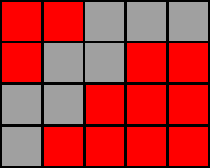
\includegraphics[width=0.52\textwidth,height=0.09\textheight]{region1}
        \caption{Input $A$}
      \end{subfigure}
      \begin{subfigure}[b]{0.45\textwidth}
        \centering
        \begin{tabular}{|p{1em}|p{1em}|p{1em}|p{1em}|p{1em}|}
          \hline
          1&2&3&4&5\\ \hline
          6&7&8&9&10\\ \hline
          11&12&13&14&15\\ \hline
          16&17&18&19&20\\  \hline
        \end{tabular}
        \caption{$B$, such that $B_{ij}=iY+j$}
      \end{subfigure}
      \begin{subfigure}[b]{0.45\textwidth}
        \centering
        \begin{tabular}{|p{1em}|p{1em}|p{1em}|p{1em}|p{1em}|}
          \hline
          1&2&0&0&0\\ \hline
          6&0&0&9&10\\ \hline
          0&0&13&14&15\\ \hline
          0&17&18&19&20\\  \hline
        \end{tabular}
        \caption{ $C^0_{ij}=A_{ij}\cdot B_{ij}$}
      \end{subfigure}
      \begin{subfigure}[b]{0.45\textwidth}
        \centering
        \begin{tabular}{|p{1em}|p{1em}|p{1em}|p{1em}|p{1em}|}
          \hline
          6&2&0&0&0\\ \hline
          6&0&0&14&15\\ \hline
          0&0&18&19&20\\ \hline
          0&18&18&19&20\\  \hline
        \end{tabular}
        \caption{$C^{t+1}_{ij}=max\left(C^t_{ij},nbr(C^t_{ij})\right)$ for $C^t_{ij} \neq 0$}
      \end{subfigure}
      \begin{subfigure}[b]{0.45\textwidth}
        \centering
        \begin{tabular}{|p{1em}|p{1em}|p{1em}|p{1em}|p{1em}|}
          \hline
          6&6&0&0&0\\ \hline
          6&0&0&20&20\\ \hline
          0&0&20&20&20\\ \hline
          0&20&20&20&20\\  \hline
        \end{tabular}
        \caption{The final result, when $C^{t+1} = C^t$}
      \end{subfigure}
      \begin{subfigure}[b]{0.45\textwidth}
        \centering
        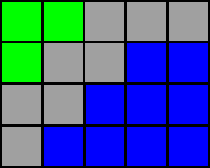
\includegraphics[width=0.52\textwidth, height=0.09\textheight]{region2}
        \caption{A colour representation of the regions}
      \end{subfigure}
      \caption{A simplistic region detection algorithm in action. $nbr(x_{ij}$ is a list of the nearest neighbours of $x_{ij}$}
      \label{simpleregion}
    \end{figure}
\end{document}
